
\documentclass{article}

\usepackage{hyperref}
\usepackage{graphicx}
\usepackage{amsmath} 
\usepackage{amssymb}
\usepackage[affil-it]{authblk}

\title{Cubical Complexes} % Sets article title
\author{Enei Sluga, Simon Hehnen} % Sets authors name
\affil
{
    Faculty of Computer and Information Science \\
    University of Ljubljana % Your institution for the title page
}
\date{\today} % Sets date for date compiled

\begin{document}
    \maketitle
    \section{Introduction}\label{sec:intro}
    In computational analysis, many datasets are naturally discrete and arranged in a grid-like structure.
    Examples include images and videos, where data is represented as pixels organized on a two-dimensional grid.
    When examining the structure of such datasets and constructing a simplicial complex,
    traditional triangulation methods may not always be the most effective.
    Instead, treating pixels as the fundamental building blocks can provide a more practical alternative.
    
    A key advantage of this approach is that, unlike the floating-point computations often required in triangulations,
    we work with discrete coordinates on a grid. This discretization offers computational benefits,
    as cubical complexes can be constructed in a fixed, ordered manner, potentially making them more
    efficient than triangulation-based methods.
    
    \section{Generating Cubical Complexes}\label{sec:generation}
    From the script, we know that a cubical complex $K$ on an $n \times n$ grid is a collection of cubes where,
    if $\sigma \in K$ and $\tau \subseteq \sigma$, then $\tau \in K$ as well. Here, $n \in \mathbb{N}$
    represents the number of squares along each side of the grid.
    Thus, the collection of all simplices has the following characteristics:
    \begin{itemize}
        \item \textbf{0-dimensional cubes:} $(n+1)^2$ vertices.
        \item \textbf{1-dimensional cubes:} $2n(n+1)$ edges.
        \item \textbf{2-dimensional cubes:} $n^2$ squares.
    \end{itemize}
    
    Instead of storing the elements of the cubical complex as a list of vertices,
    we can utilize the inherent grid structure. For a two-dimensional grid,
    each cube can be assigned coordinates $(x, y)$, where $x, y \in \{0, 1, 2, \dots, 2n\}$.
    By superimposing the coordinate axes over the original $n \times n$ grid (see Figure \ref{fig:dia2d}),
    the coordinates $(x, y)$ correspond to the cube whose center is located at $(x, y)$.
    We further define the orientations as follows:
    \begin{itemize}
        \item Each square is oriented with its vertices ordered in a counterclockwise (positive rotational) direction.
        \item Vertical edges are oriented upwards, and horizontal edges are oriented to the right.
    \end{itemize}
    
    This coordinate assignment has the following properties (refer to Figure \ref{fig:dia2d}):
    \begin{itemize}
        \item If $x$ and $y$ are both odd, then $(x, y)$ represents a square.
        \item If exactly one of $x$ or $y$ is odd, then $(x, y)$ represents an edge.
        \item If $x$ and $y$ are both even, then $(x, y)$ represents a vertex.
    \end{itemize}
    
    \begin{figure}\label{fig:dia2d}
        \centering
        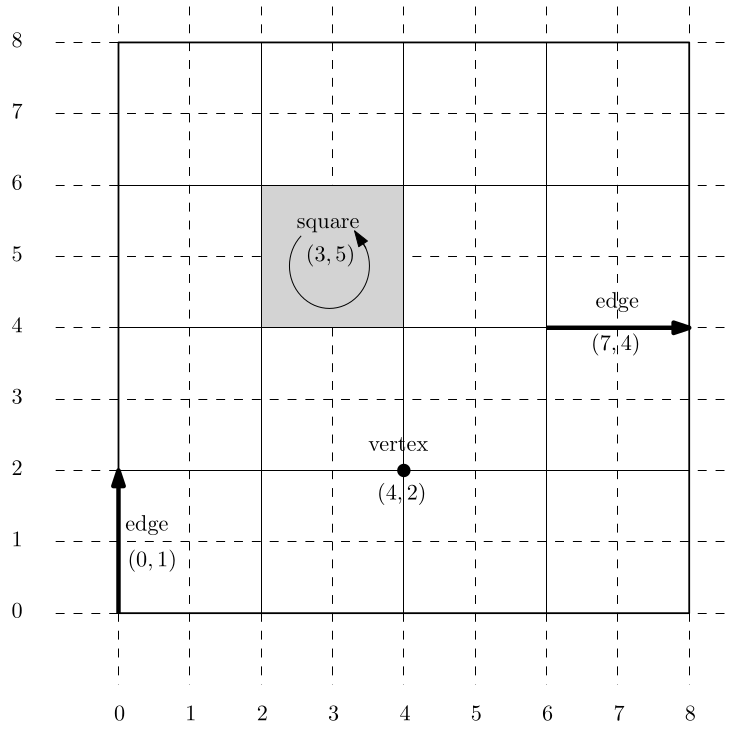
\includegraphics[width=0.5\textwidth]{dia2d.png}
        \caption{TODO}
    \end{figure}
    
    This method extends naturally to higher dimensions.
    For instance, in a 3D grid, a square $(x, y, z)$ will have exactly two even coordinates and one odd coordinate.
    
    \section{Visualize the Cubical Complex}\label{sec:vis}
    To visualize a cubical complex as described in Section \ref{sec:intro},
    we need to adjust the calculations to decode the encoded coordinates.
    For instance, the vertices were all doubled during encoding because they only
    have even labels.

    To determine the boundary vertex coordinates from an edge, we divide the even coordinates by two.
    Then, for the odd label, we calculate the boundary coordinates by adding and subtracting one from it.

    This method naturally scales to higher dimensions. In higher-dimensional objects,
    we follow the same process, calculating more boundary coordinates as there are more odd labels to consider.

    Using this approach, we can effectively visualize a cubical complex encoded in this specific format.

    \section{Computing Homology}
    TODO explain how homolgy is computed

    \section{Persistent Homology}
    To calculate persistent homology for our cubical complexes,
    we first need to define a filter function. This function allows us to
    create different complexes from the same initial grid, each with distinct properties.

    \subsection{The Filter Function}\label{subsec:filter}
    The filter function works by scaling down the grid, effectively combining
    multiple vertices into one. In a 3D grid, for example, eight vertices are
    combined into a single vertex. Additionally, the function offers multiple
    options for labeling the resulting vertex. These options include:
    \begin{itemize}
        \item \textbf{Majority}: The new vertex inherits the label that occurs most frequently among the surrounding vertices.
        \item \textbf{Max}: The new vertex takes the maximum label from the surrounding vertices.
        \item \textbf{Min}: The new vertex takes the minimum label from the surrounding vertices.
        \item \textbf{Random}: A label is randomly selected from the surrounding vertices.
    \end{itemize}

    For our test object, we chose the \textbf{max} method
    This means the new vertex inherits the maximum label from the surrounding eight vertices.
    If any of the surrounding vertices is labeled as $1$, the resulting vertex is also labeled as $1$.

    \subsection{Results for Persistant Homology}\label{subsec:resultsPers}
    TODO show diagrams, the interesting object and stuff.
    
    \section{Conclusion}
    TODO Conclusion

    \section{Division of Work}
    Simon did the code for the creation of cubical complexes and did the visualization.
    Enei provided the code for Homology computation.
    Persistant Homology was done by both together with the examples.

    \section{Bibliography}*
    We used the section on cubical complexes from the lecture script (P.106-108).

\end{document}
